\documentclass[11pt]{article}

\usepackage{a4wide}
\usepackage{mathptm}
\usepackage{xspace}
\usepackage{amsmath}
\usepackage{graphicx}
\usepackage{algorithm}
\usepackage{algpseudocode}
\usepackage{tikz}
\usepackage{tkz-graph}
\usetikzlibrary{shapes.misc, positioning}
\usepackage{listings}
\usepackage{color}
\usepackage{hyperref}
\usepackage{graphicx} % For table

\definecolor{dkgreen}{rgb}{0,0.6,0}
\definecolor{gray}{rgb}{0.5,0.5,0.5}
\definecolor{mauve}{rgb}{0.58,0,0.82}

\lstset{frame=tb,
  language=Java,
  aboveskip=3mm,
  belowskip=3mm,
  showstringspaces=false,
  columns=flexible,
  basicstyle={\small\ttfamily},
  numbers=left,
  numberstyle=\tiny\color{gray},
  keywordstyle=\color{blue},
  commentstyle=\color{dkgreen},
  stringstyle=\color{mauve},
  breaklines=true,
  breakatwhitespace=true,
  tabsize=3
}
\begin{document}

\title{Implementing Secure Authentication: A Comparison of OAuth 2.0 and Basic Authentication}

\author{Kristian E. Takvam and Lars Magnus Nordeide}

\maketitle

\begin{abstract}
%Abstract: 10-15 lines with the software technology and the highlights from the project that has been undertaken.
This project focuses on designing and building FeedApp, a web application that allows users to create and participate in surveys and polls. The app is developed using a modern technology stack, with OAuth 2.0 integrated for secure user authentication and token-based authorization, ensuring a safe and smooth experience for users. The backend is powered by Spring Boot and Spring Web MVC, providing a reliable RESTful API, while the frontend, built with Svelte and Vite, delivers a fast and responsive Single Page Application (SPA).

The application is based on a well-structured domain model that defines the relationships between key entities like users, surveys, polls, and votes. PostgreSQL and MongoDB are used to handle structured and unstructured data effectively, and RabbitMQ is included for efficient communication between different parts of the system. The use of Docker helps with deployment and scalability, making it easier to manage and run the application in different environments.

As part of this project, an evaluation was conducted to compare OAuth 2.0 with Basic Authentication and API Keys. Experiments were run to test scalability, ease of implementation, and security. The results showed that OAuth 2.0 performs better in handling high user loads, provides advanced security features like token expiration and scope control, and is flexible enough to work well with third-party systems. These findings make OAuth 2.0 an excellent choice for scalable and secure web applications.

Overall, this project highlights how a modern, scalable architecture can provide a secure and user-friendly platform for collaborative participation in surveys and polls. It demonstrates the importance of choosing the right technologies to ensure both performance and security in web application development.

\end{abstract}

%\input{commands}

\section{Introduction}
\label{sec:introduction}

% A brief introduction to the prototype implementation and topic of the project.
The FeedApp project seeks to develop a running prototype of a full-stack FeedApp. The purpose of this application is to allow users to create and manage polls and surveys. Registered users can also vote on polls using a web-based user interface. 
\medskip

% Discuss (briefly) the technology stack that has been selected
\noindent
The technology stack is as follows:
\begin{itemize}
\item Java with SpringBoot as the general platform/framework,
\item Spring Web MVC for implementing a HTTP/REST AP,
\item Svelte + Vite for implementing a Single Page App user interface,
\item Jakarta Persistence API with Hibernate and Postgres for implementing object-relational database mapping,
\item MongoDB as a non-relational database,
\item RabbitMQ as a message broker,
\item Docker as a container engine.
\item OAuth 2.0: The chosen authentication protocol ensures secure user authentication and authorization, providing a scalable and standard mechanism to handle access control. We will be conducting a technology assessment according to Brown and Walnau.\cite{brown:96}
\end{itemize}

% A brief account of the results that have been obtained in the project.
\noindent
 *A brief account of the results that have been obtained in the project.*
\medskip

% A one paragraph overview at the end, explaining how the rest of the report is / has been organised.
\noindent
This rest of this report is organised as follows:

Section~\ref{sec:design} gives a detailed descprition about the functional aspects of the FeedApp application. This includes use cases, domain model and an application flow diagram.

Section~\ref{sec:technology} documents the experiments conducted, following the methodology described in the paper by Brown and Walnau.

Section~\ref{sec:implementation} gives a brief explanation of how the prototype has been implemented. It provides details to those who may want to run the application and how they may develop it further.


\section{Design}
\label{sec:design}

% Around 5 pages about functional aspects of the FeedApp application.
The main purpose of the FeedApp is to deliver a modern web application that offers a seamless and intuitive experience, allowing users to log in, craft their own surveys and cast votes on existing polls.

\subsection{Use cases}
 \textbf{User Authentication and Authorization}:
In FeedApp, user authentication and authorization are handled using OAuth 2.0 to make logging in secure and easy. When users want to log in, they can either use their FeedApp credentials or sign in through a trusted service like Google. If they choose a third-party login, they are redirected to that provider to confirm their identity. Once they’re logged in, the system gives them a token that lets them interact with the app without having to log in again for every action. This keeps things secure and makes the whole experience smoother for the user.
\medskip

\noindent
 \textbf{Survey Creation}:
One of the main features of FeedApp is letting users create surveys. After logging in, users can go to the "Create Survey" page to start building their survey. First, they give the survey a title. Then they can add multiple polls to it, setting the order of each poll so that everything flows the way they want. Inside each poll, they can add as many options as needed for participants to choose from. Once the user is done creating their survey, it gets saved in the system and is ready for others to participate in. This makes it simple to create detailed surveys with multiple questions and options.
\medskip

\noindent
 \textbf{Voting on polls}:
Voting is another important part of FeedApp. Logged-in users can find active surveys, go through the polls, and select the options they want to vote for. Once they’ve made their choices, they submit their votes, and the system processes them. After the vote is recorded, the results are updated in real time so everyone can see the latest vote counts. This real-time feature makes the app more interactive and lets participants stay up-to-date on how the survey is doing.
\medskip

\noindent
 \textbf{View Survey Results}:
FeedApp also makes it easy to view survey results, both for the person who created the survey and for the people who participated in it. After a survey is published, users can look at the results for each poll. The app shows things like the total number of votes and how the votes are spread across the different options. These results update automatically whenever new votes are added, so the data is always current. This feature helps creators see how their surveys are performing and gives participants a clear view of the outcome.

\begin{figure}[thb]
	\centering
	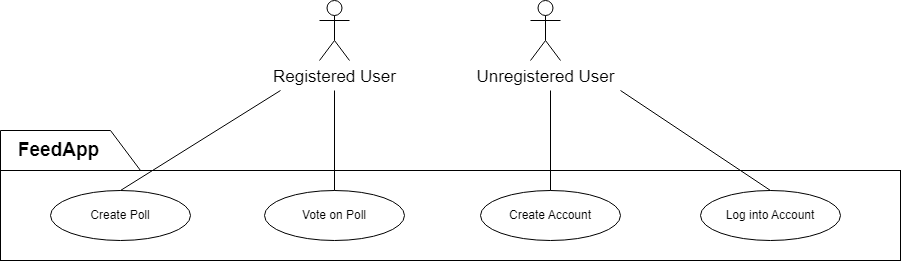
\includegraphics[scale=0.5]{figs/usecase.png}
	\caption{Use Case}
	\label{fig:usecase}
\end{figure}

\subsection{Domain model}
\begin{figure}[!htbp]
	\centering
	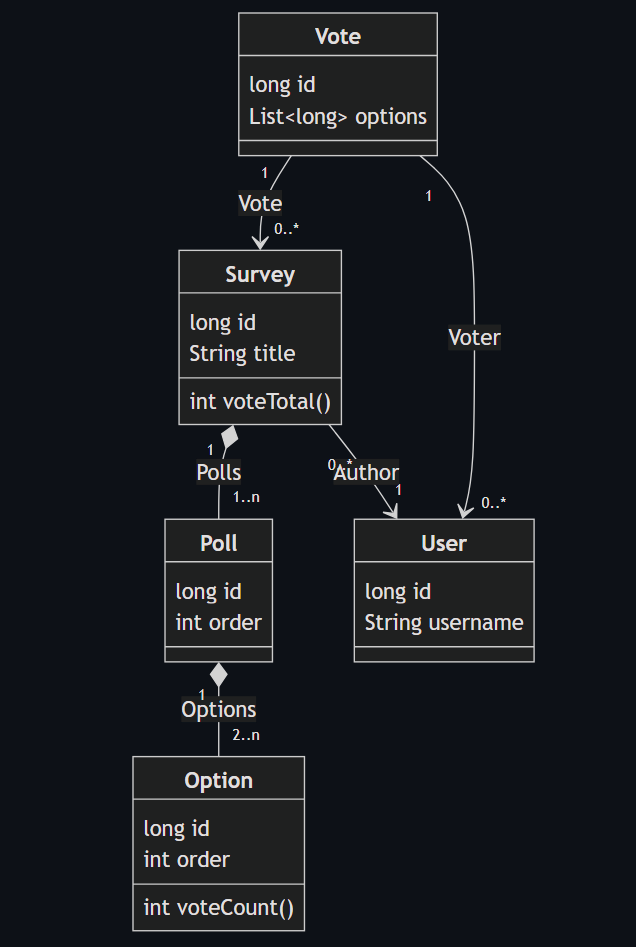
\includegraphics[scale=0.5]{figs/domainmodel.png}
	\caption{The Domain Model.}
	\label{fig:domainmodel}
\end{figure}
The domain model for the FeedApp application captures the core entities and their relationships, providing the foundation for managing surveys, polls, and user interactions. This model ensures a structured and scalable approach to data representation, supporting the application's primary functions such as survey creation, voting, and user management.
\medskip

\subsubsection*{Entities in the Domain Model}

The following entitites can be seen in figure~\ref{fig:domainmodel}:
\smallskip

\noindent
 \textbf{User}:
A User represents an individual interacting with the system, either as a participant in surveys or as an author creating new polls. The Survey entity acts as the central object, representing a collection of polls authored by a user. Each survey is comprised of one or more Polls, which in turn consist of multiple Options that users can select from when casting their votes. The Vote entity captures the act of participation, linking users with the options they select in a given poll.
\medskip

\noindent
 \textbf{Survey}:
A Survey is the primary container entity, representing a collection of polls authored by a user. Each survey has a unique id and a title describing its purpose. The voteTotal() method calculates the total number of votes across all associated polls, providing a quick summary of survey engagement.
\medskip

\noindent
 \textbf{Poll}:
The Poll entity is a component of a survey, representing a single voting instance within it. Polls are ordered using the order attribute, ensuring that their sequence within a survey can be maintained. Each poll is linked to multiple options, allowing users to select from predefined choices.
\medskip

\noindent
 \textbf{Option}:
Options are individual choices within a poll. Each option is uniquely identified by an id and has an associated order attribute to define its position within the poll. The voteCount() method calculates the number of votes an option has received, enabling detailed poll result analysis.
\medskip

\noindent
 \textbf{Vote}:
The Vote entity captures user participation in polls. A vote links a user to specific survey options they have chosen, ensuring accurate representation of voting behavior. The entity includes a unique id and relationships with the User, Survey, and Option entities.
\medskip

\noindent
\subsubsection*{Relationships}
\noindent
The relationships between these entities are key to the domain model's functionality. A survey can have many polls, and each poll must have at least two options to be valid. Votes are associated with both users and surveys, reflecting the choices made by participants. This model not only reflects the application's functional requirements but also ensures data integrity through these defined relationships. Additionally, the use of attributes such as timestamps and unique identifiers allows for detailed analytics and user tracking, which are essential for the platform's growth and adaptability.
\medskip

\noindent
This domain model provides a solid foundation for implementing the core features of FeedApp, including survey creation, user participation, and vote aggregation. Its design ensures that the application can scale to accommodate a growing number of users and complex interactions, while maintaining a clear and manageable structure.

\subsection{Architecture}
\begin{figure}[!htbp]
	\centering
	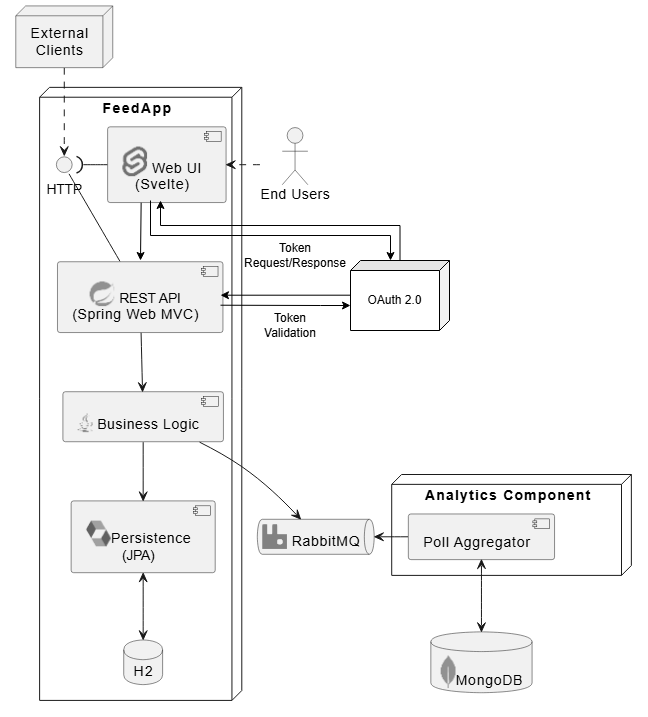
\includegraphics[scale=0.5]{figs/architecture.png}
	\caption{Architecture}
	\label{fig:architecture}
\end{figure}

The architecture of FeedApp, shown in Figure~\ref{fig:architecture}, follows a modular, layered design. It includes a frontend, backend, and supporting infrastructure, all working together to provide a secure and scalable application.

The frontend, built with Svelte, offers users a fast and responsive interface for interacting with surveys. This Single Page Application (SPA) communicates with the backend using HTTP requests and includes OAuth 2.0 token-based authentication to keep interactions secure.

The backend is implemented using Spring Boot. It provides a RESTful API through Spring Web MVC, which handles requests from the frontend and coordinates with the business logic and persistence layers. Core functionalities, such as survey and vote management, are handled in this layer.

The persistence layer uses both PostgreSQL and MongoDB. PostgreSQL stores structured data like users, surveys, polls, and votes, ensuring data consistency. MongoDB handles unstructured or semi-structured data, such as analytics and logs, allowing flexible queries.

RabbitMQ, a message broker, enables communication between components and supports asynchronous tasks like vote aggregation. This design ensures the system can handle high loads efficiently.

Security is a core focus, with OAuth 2.0 providing robust user authentication and authorization. Tokens issued by an external or custom Authorization Server are used to validate user identities and enforce access controls.

This layered design makes FeedApp modular, easy to maintain, and scalable. It is well-suited for the current requirements and provides a strong foundation for future improvements.



%%%%
\subsubsection{OAuth 2.0: How It Works (Google Implementation)}
OAuth 2.0 is a framework that allows secure access to user resources without exposing their credentials. It is widely used for authenticating users and authorizing API calls, and Google’s implementation is one of the most commonly used examples.

Figure~\ref{fig:oauth2-google} illustrates the sequence of interactions in an OAuth 2.0 flow, specifically using Google's implementation. Here's a step-by-step explanation of the process:
\begin{enumerate}
\item \textbf{Request Token}:
The user begins by interacting with the FeedApp (referred to as "Your JS App" in the figure) and initiates the login process. The application sends a request to Google’s servers to obtain an authorization token.

\item \textbf{User Login and Consent}:
Google then prompts the user to log in and provide consent for the requested scopes (permissions). These scopes define what the application is allowed to access on the user's behalf, such as their profile or email address.

\item \textbf{Token Response}:
Once the user consents, Google generates and returns an Access Token to the application. This token represents the user’s identity and their permissions.

\item \textbf{Validate Token}:
Before making API requests, the application can validate the token with Google’s servers to ensure it is legitimate and has not expired. This step ensures an additional layer of security.

\item \textbf{Use Token to Call Google API}:
After validation, the application can use the token to securely call Google’s APIs or perform other operations. The token is included in the Authorization header of API requests.
\end{enumerate}

This flow highlights the key advantage of OAuth 2.0: the user's credentials are never directly shared with the application, reducing security risks. Instead, a short-lived token is used, which can be revoked or scoped as needed \cite{google:oauth}.

\begin{figure}[htbp]
\centering
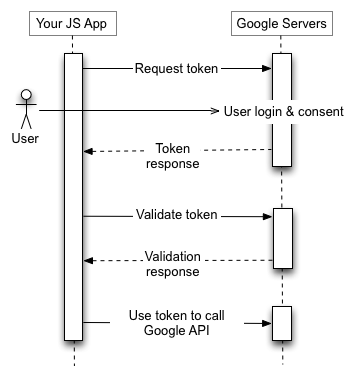
\includegraphics[scale=0.5]{figs/OAuthGoogle.png}
\caption{OAuth 2.0 Flow with Google Implementation.}
\label{fig:oauth2-google}
\end{figure}

Security and Benefits
OAuth 2.0's token-based approach is highly secure, as tokens can be limited in scope and validity. Google’s implementation also ensures strong user consent flows, making it suitable for applications requiring sensitive data access. For FeedApp, this implementation guarantees that only authenticated and authorized users can create surveys, cast votes, and access results.

This explanation is based on official documentation from Google Developers, which provides further detai



\section{Technology Assessment}
\label{sec:technology}

This section explores the key concepts, architecture, and performance characteristics of the chosen authentication technologies: OAuth 2.0 and Basic Authentication. These technologies are evaluated in the context of FeedApp, a system designed to facilitate secure interactions such as creating polls, voting, and managing user-generated content. The primary objective is to assess the scalability and performance of these methods under varying load conditions, ensuring FeedApp's reliability and user experience.

Figure~\ref{fig:framework}, adapted from \cite{brown:96}, provides an overview of the framework used for this evaluation. This structured approach ensures a thorough assessment of both technologies based on their architectural foundations and real-world performance.

\begin{figure}[thb]
	\centering
	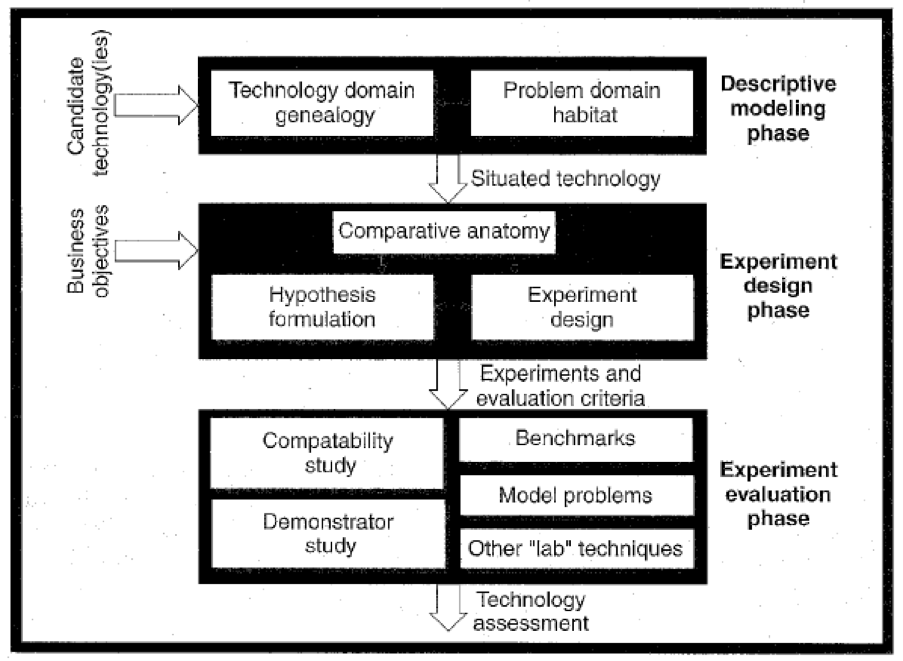
\includegraphics[scale=0.5]{figs/framework.png}
	\caption{Software technology evaluation framework.}
	\label{fig:framework}
\end{figure}

\subsection{Descriptive Modeling}
OAuth 2.0 has become the industry standard for secure API access, with implementations by platforms such as Google \cite{oauthnet,google:oauth}. It enables systems to delegate access by issuing short-lived access tokens to clients instead of directly sharing user credentials. This token-based approach enhances security by limiting what resources can be accessed and for how long. For instance, in our FeedApp, OAuth 2.0 can be used to ensure that only authenticated users can vote or create surveys, without exposing sensitive data like passwords. It is commonly used by large platforms like Google and Facebook, making it an industry standard for secure APIs.

On the other hand, Basic Authentication is a simpler method where the username and password are included in every request’s header for authentication. Although this method is straightforward to implement, it comes with significant security risks, such as the exposure of credentials in every request, as noted in OWASP’s Authentication Cheat Sheet \cite{owasp:authcheatsheet}.. There is no inherent mechanism to restrict access or enforce expiration policies. This simplicity makes Basic Authentication suitable for smaller-scale systems or those that are not exposed to public internet traffic.

The purpose of this evaluation is to compare these two technologies in the context of FeedApp and determine whether the additional complexity of OAuth 2.0 is justified for its intended use cases.

\subsection{Experiment Design}
To evaluate the two technologies, we designed experiments that focused on three main hypotheses. First, we hypothesized that Basic Authentication would provide lower average request durations due to its simplicity and better throughput under moderate loads. This expectation was based on its lightweight nature and lack of cryptographic overhead. Second, we anticipated that OAuth 2.0 would outperform Basic Authentication in terms of scalability under higher loads. Token-based systems like OAuth 2.0 are generally recognized as more scalable compared to Basic Authentication in high-load environments due to their stateless architecture. Third, we expected that both methods would experience failures under extreme concurrency but that OAuth 2.0 would fail more gracefully due to its token-based architecture.
\subsubsection*{Experiment Setup and Tools}
The experiments involved simulating various levels of concurrent users, ranging from 50 to 10,000, accessing a protected API endpoint. These requests were designed to replicate real-world interactions, such as retrieving data or performing secure operations. Key metrics, including average request duration, failure rates, and throughput, were recorded to evaluate each method’s performance and scalability.

For initial testing and validation of the API functionality, Postman was used to manually verify that the endpoints were behaving as expected. Following this, Newman, the command-line interface (CLI) version of Postman, was employed to automate test script execution. Newman allowed us to measure key metrics such as response times, failure rates, and data throughput under moderate loads, specifically scenarios with up to 100 virtual users.

As the need to simulate higher concurrency arose, K6 was introduced as the primary load testing tool. K6 enabled the simulation of up to 10,000 concurrent users and provided detailed metrics such as average request durations, failure rates, and system throughput. Custom scripts were written in JavaScript for K6 to implement both Basic Authentication and OAuth 2.0 flows. These scripts primarily tested the \texttt{/api/protected} endpoint, which required valid authentication for access. The tests captured key performance indicators, including latency and the system’s ability to handle extreme loads.

The FeedApp backend was deployed locally for all experiments, running on a Spring Boot server with a PostgreSQL database for structured data storage. For the OAuth 2.0 tests, Google’s Authorization Server was used for issuing and validating tokens, ensuring a real-world implementation of this authentication method. 

\subsubsection*{Hypotheses}
The primary goals of this assessment are to compare the performance metrics of Basic Authentication and OAuth 2.0, including average request durations, failure rates, and data overhead. Assess the scalability of each method under increasing load. Provide recommendations for scenarios where each technology would be most effective.

\begin{enumerate}
    \item \textbf{Hypothesis 1}: Performance: Basic Authentication will demonstrate lower average request durations and better throughput under moderate loads due to its simplicity and minimal computational overhead.
    \item \textbf{Hypothesis 2}: Scalability: OAuth 2.0, with its stateless token validation, will outperform Basic Authentication at higher loads by avoiding database contention.
    \item \textbf{Hypothesis 3}: Failure Rates: Both methods will experience failure rates under extreme concurrency, but OAuth 2.0 will fail more gracefully due to its architecture.
\end{enumerate}

\subsection{Experiment Evaluation}
The experimental results provided valuable insights into the strengths and limitations of both authentication methods. At lower loads, both OAuth 2.0 and Basic Authentication performed well, with no significant differences in metrics such as average request durations or failure rates. However, as concurrency increased, clear differences began to emerge.

Basic Authentication demonstrated faster response times and better throughput under moderate loads, owing to its simple design that requires fewer computational steps. However, its reliance on a centralized database for validating credentials became a bottleneck as the number of concurrent users grew. This dependency led to higher latencies and increased failure rates under heavy loads, particularly beyond 1000 virtual users.

In contrast, OAuth 2.0 showed consistent performance up to moderate loads by leveraging its stateless architecture, which avoids frequent database interactions. However, the cryptographic operations required for token validation introduced additional overhead, resulting in higher average request durations. Under extreme concurrency (10,000 virtual users), OAuth 2.0 also experienced significant failures due to resource exhaustion during token validation.

Tables~\ref{tab:performance-comparison} and \ref{tab:scalability-results} summarize the key findings. Table~\ref{tab:performance-comparison} highlights the results for 100 virtual users, showing comparable performance between the two methods. Table~\ref{tab:scalability-results}, however, demonstrates the challenges both methods faced at 3000 virtual users, with Basic Authentication achieving higher throughput but struggling with scalability and OAuth 2.0 encountering significant resource constraints.

\begin{table}[h!]
\centering
\resizebox{\textwidth}{!}{%
\begin{tabular}{|l|c|c|p{6cm}|}
\hline
\textbf{Metric} & \textbf{Basic Authentication (100 VUs)} & \textbf{OAuth 2.0 (100 VUs)} & \textbf{Observations} \\ \hline
\textbf{Data Received (kB/s)}  & 447 kB (15 kB/s)          & 447 kB (15 kB/s)              & Equal amount of data received for both methods.  \\ \hline
\textbf{Data Sent (kB/s)  } & 1.8 MB (61 kB/s)          & 204 kB (6.7 kB/s)             & OAuth sends more data due to token size and overhead.   \\ \hline
\textbf{Average Request Duration (ms)} & 9.96 ms                  & 3.95 ms                       & OAuth takes ~2.5x longer due to token validation overhead.  \\ \hline
\textbf{Minimum Request Duration (µs)} & 504.6 µs                 & 93 µs                         & Basic Auth has a faster minimum response time.            \\ \hline
\textbf{Maximum Request Duration (ms)} & 210.48 ms                & 44.66 ms                      & OAuth has significantly higher maximum response times.  \\ \hline
\textbf{95th Percentile (ms) }  & 22.12 ms                 & 19.84 ms                      & OAuth shows slightly higher tail latency.          \\ \hline
\textbf{Failed Requests } & 0\%                       & 0\%                            & Both methods handled the load without failures.   \\ \hline
\textbf{Requests per Second   }   & 49.31                    & 49.61                         & Throughput is similar for both methods.     \\ \hline
\end{tabular}
}
\caption{Performance Comparison for 100 Virtual Users}
\label{tab:performance-comparison}
\end{table}

\subsubsection*{Scalability Results}

At higher loads, significant differences were observed. Table~\ref{tab:scalability-results} summarizes the scalability test results for Basic Authentication and OAuth 2.0 under extreme loads.



\begin{table}[h!]
\centering
\resizebox{\textwidth}{!}{%
\begin{tabular}{|l|c|c|c|}
\hline
\textbf{Metric}                      & \textbf{Basic Authentication (3000 VUs)} & \textbf{OAuth 2.0 (3000 VUs)} & \textbf{Observations} \\ \hline
\textbf{Average Request Duration}    & 1.19 s                                  & 1.68 s                        & OAuth has higher overhead under load. \\ \hline
\textbf{Failure Rate}                & 5.83\%                                  & 12.11\%                       & OAuth fails more frequently due to resource exhaustion. \\ \hline
\textbf{Requests per Second}         & 1241.61 req/s                           & 940.98 req/s                  & Basic Auth achieves higher throughput. \\ \hline
\textbf{90th Percentile Latency}     & 1.52 s                                  & 2.31 s                        & OAuth has significantly worse tail latency. \\ \hline
\end{tabular}
}
\caption{Scalability Test Results for 3000 Virtual Users}
\label{tab:scalability-results}
\end{table}

\subsubsection*{Observations}
The results of the experiments provided a clear view of how each technology behaves under different conditions. At lower loads, both methods performed well, with minimal differences in average request durations and no failures. Basic Authentication demonstrated slightly faster response times due to its straightforward design, which requires fewer computational steps than OAuth 2.0’s token validation process.

However, as the number of concurrent users increased, differences began to emerge. At 200 to 1000 virtual users, Basic Authentication started to show signs of strain due to its reliance on a centralized database for credential validation. This dependency created bottlenecks as the number of requests grew. In contrast, OAuth 2.0 maintained consistent performance up to 1000 users by leveraging its stateless architecture, which does not require constant interaction with a database.

When the load was increased to extreme levels, such as 3000 and 10,000 concurrent users, both methods experienced significant challenges. Basic Authentication faced severe scalability issues, with failure rates exceeding 75\% at 10,000 users. The database became overwhelmed, leading to high latencies and frequent timeouts. OAuth 2.0, on the other hand, faced bottlenecks in token validation. Although it avoided database contention, the cryptographic operations required for validating tokens proved to be resource-intensive. This resulted in a 100\% failure rate at 10,000 users, indicating that the system was unable to handle such extreme loads without optimization.

Overall, the results show that while Basic Authentication is faster and simpler at low loads, it struggles to scale effectively. OAuth 2.0 offers better scalability at moderate loads but requires additional resources to handle extreme concurrency.




\section{Prototype Implementation}
\label{sec:implementation}

This section should provide brief details of how the prototype has been implemented.
You may want to use come code snippets here, but only focus on core features and aspects.
You are not meant to copy/paste your whole application code into the report.
Focus for instance how other developers may run your application and how they might develop it further...


SurveyController.java can be seen as shown in Figure~\ref{fig:surveycontroller}.


\begin{figure}[!htbp]
	\lstinputlisting[language=java, firstline=22, lastline=32]{code/SurveyController.java}
	\caption{SurveyController}
	\label{fig:surveycontroller}
\end{figure}


\section{Conclusions}

Concludes on the project, including the technology, its maturity,
learning curve, and quality of the documentation.

The references used throughput the report should constitute a well
chosen set of references, suitable for someone interesting in learning
about the technology.


\bibliographystyle{plain}
\bibliography{report.bib}{}

\end{document}
